% =====================================================================
% An Empirical Comparison of Parameter-Efficient Mitigation Strategies
% for Catastrophic Forgetting in Small LLMs under Compute-Constrained
% Continual Fine-Tuning
%
% IEEE Conference template (IEEEtran, 2-column, conference mode)
% Build: pdflatex main && bibtex main && pdflatex main && pdflatex main
% =====================================================================
\documentclass[conference]{IEEEtran}
\IEEEoverridecommandlockouts

% ---------- Packages ----------
\usepackage{cite}
\usepackage{amsmath,amssymb,amsfonts}
\usepackage{algorithmic}
\usepackage{algorithm}
\usepackage{graphicx}
\usepackage{textcomp}
\usepackage{xcolor}
\usepackage{booktabs}
\usepackage{multirow}
\usepackage{array}
\usepackage{hyperref}
\usepackage{url}
\usepackage{tikz}
\usepackage{pgfplots}
\pgfplotsset{compat=1.17}

% ---------- Macros ----------
\newcommand{\method}[1]{\textsc{#1}}
\newcommand{\dataset}[1]{\textsc{#1}}
\newcommand{\mmr}{\textsc{MMR}}
\newcommand{\todo}[1]{\textcolor{red}{[TODO: #1]}}

\def\BibTeX{{\rm B\kern-.05em{\sc i\kern-.025em b}\kern-.08em
    T\kern-.1667em\lower.7ex\hbox{E}\kern-.125emX}}

\begin{document}

\title{An Empirical Comparison of Parameter-Efficient Mitigation\\
Strategies for Catastrophic Forgetting in Small LLMs under\\
Compute-Constrained Continual Fine-Tuning}

\author{
\IEEEauthorblockN{Gautam Dubey}
\IEEEauthorblockA{Department of Computer Science \& Engineering\\
Medicaps University\\
Indore, India\\
Email: gautamdubey296@gmail.com}
}

\maketitle

% ---------- Abstract ----------
\begin{abstract}
Catastrophic forgetting (CF) remains a central obstacle to deploying
Large Language Models (LLMs) in settings where new tasks arrive
sequentially. While recent work has produced a broad zoo of
mitigation strategies---ranging from elastic-weight regularization
and experience replay to orthogonal low-rank adapters---almost all
evaluations are performed on 7B--13B-parameter models trained on
data-center-grade hardware. In this work we ask a different but
equally important question: \emph{which mitigation strategies remain
effective when the practitioner is restricted to a sub-2B parameter
model and a single free-tier GPU?} We present a systematic empirical
comparison of six representative strategies---full fine-tuning,
vanilla LoRA, LoRA with Elastic Weight Consolidation (EWC),
LoRA with Experience Replay, Orthogonal LoRA (O-LoRA), and a
\emph{Minimal Mixed Rehearsal} (MMR) recipe we formalize from a
recent empirical observation---applied to Qwen2.5-1.5B-Instruct and
Phi-3.5-mini-instruct across a four-task sequence drawn from GLUE
(SST-2 $\rightarrow$ MRPC $\rightarrow$ CoLA $\rightarrow$ MNLI).
All experiments are run under QLoRA 4-bit quantization on a single
NVIDIA T4. We report Average Accuracy, Forgetting, Backward Transfer,
wall-clock training time, and peak GPU memory, and visualize the
resulting accuracy/compute trade-off as a Pareto frontier.
Our results show that \todo{insert one-sentence headline finding once
results are in}, and that MMR with a replay fraction as low as
\todo{X\%} matches or exceeds heavier methods while incurring
negligible additional compute. We release all code, configurations,
and run logs to enable reproduction on free-tier hardware.
\end{abstract}


\begin{IEEEkeywords}
catastrophic forgetting, continual learning, large language models,
parameter-efficient fine-tuning, LoRA, QLoRA, rehearsal
\end{IEEEkeywords}

% ---------- Body ----------
\section{Introduction}
\label{sec:introduction}

Large Language Models (LLMs) have become the default substrate for
modern natural language processing, but the prevailing usage pattern
treats each fine-tuned model as a single static artifact. In
practice, downstream tasks rarely arrive simultaneously: a model
deployed in a research group, startup, or product team is repeatedly
asked to acquire \emph{new} capabilities (a new domain, a new
language, a new instruction style) without losing the capabilities it
already possesses. This is the classical setting of
\emph{continual learning}, and the failure mode it exposes---a sharp
collapse in performance on previously mastered tasks the moment a new
task is introduced---is \emph{catastrophic forgetting} (CF)
\cite{mccloskey1989catastrophic,luo2023empirical}.

The recent CF-mitigation literature for LLMs is wide and
fast-moving. Regularization-based methods penalize movement of
important parameters \cite{kirkpatrick2017overcoming,li2024revisiting,song2025hierarchical};
rehearsal-based methods reintroduce data
from earlier tasks during current-task training \cite{huang2024ssr,reynolds2025mixed};
architectural and PEFT-based methods isolate
task-specific knowledge in dedicated low-rank subspaces
\cite{hu2021lora,wang2023olora,fawi2024curlora,nayak2025sculpting}.
Despite the breadth of techniques, the experimental setting in which
they are typically validated is remarkably homogeneous: a
$\geq$7B-parameter base model, an A100-class GPU, and large
fine-tuning budgets. The resulting body of evidence is largely
silent on the regime that most students, independent researchers,
and small teams actually inhabit: a sub-2B-parameter base model and a
single free-tier GPU (e.g.\ an NVIDIA T4 on Colab or Kaggle).

This work fills that gap. We perform a controlled empirical
comparison of six representative CF-mitigation strategies on small,
publicly available instruction-tuned LLMs under a strict
free-tier compute envelope. Concretely, we make the following
contributions:

\begin{itemize}
    \item We establish a reproducible \emph{small-model,
    free-tier} benchmark for CF on a four-task sequence drawn from
    GLUE (SST-2 $\rightarrow$ MRPC $\rightarrow$ CoLA $\rightarrow$
    MNLI), with all six methods implemented uniformly on top of
    QLoRA 4-bit fine-tuning.

    \item We formalize \emph{Minimal Mixed Rehearsal} (MMR), a simple
    rehearsal recipe that retains only a small fraction
    ($\sim$\todo{$f\%$}) of each earlier task's training set and
    interleaves it with the current task at every optimization step.
    The recipe is parameter-free at inference time and adds
    negligible memory and wall-clock overhead.

    \item We report not only the standard continual-learning metrics
    (Average Accuracy, Forgetting, Backward Transfer) but also
    \emph{wall-clock training time} and \emph{peak GPU memory}, and
    visualize the resulting accuracy/compute trade-off as a Pareto
    frontier. This compute-aware view is, to our knowledge, missing
    from existing comparative CF studies.

    \item Across both Qwen2.5-1.5B-Instruct and Phi-3.5-mini-instruct,
    we observe that
    \todo{state the headline empirical finding once results are in,
    e.g.\ ``MMR matches O-LoRA in average accuracy while reducing
    training time by X\%''}.

    \item We release code, configurations, and run logs to enable
    end-to-end reproduction of every reported number on a single
    Colab T4 session.
\end{itemize}

The remainder of the paper is organized as follows.
Section~\ref{sec:related} situates our work in the existing CF
literature. Section~\ref{sec:method} introduces our notation,
formalizes each comparison method, and presents MMR.
Section~\ref{sec:setup} details the experimental protocol.
Section~\ref{sec:results} reports our main empirical results.
Section~\ref{sec:discussion} draws practical guidance from the
findings, and Section~\ref{sec:conclusion} concludes.

\section{Related Work}
\label{sec:related}

Catastrophic forgetting (CF), first characterized by~\cite{mccloskey1989catastrophic}, remains a
fundamental obstacle to continual learning in neural networks: sequential gradient updates cause a
model to overwrite previously acquired knowledge when it adapts to a new task distribution.
With the rise of large language models (LLMs), CF has taken on renewed urgency; practitioners
increasingly need to fine-tune pre-trained models on successive domain- or task-specific corpora
without retaining all prior training data~\cite{luo2023empirical,li2024revisiting}.
We organize the existing literature into four clusters.

% Required packages (add to main.tex preamble if missing):
%   \usepackage{booktabs}

\subsection{Regularization-Based Methods}

Regularization approaches penalize changes to model parameters that are deemed important for prior
tasks.
Elastic Weight Consolidation (EWC)~\cite{kirkpatrick2017overcoming} anchors each parameter to its
post-training value with a quadratic penalty weighted by the diagonal of the empirical Fisher
information matrix, providing a theoretically grounded stability--plasticity trade-off.
While EWC is widely adopted as a baseline, its memory cost grows linearly with the number of tasks
when the full Fisher diagonal must be stored, and the penalty strength $\lambda$ must be tuned
per task sequence.
Hierarchical regularization~\cite{song2025hierarchical} extends the EWC idea to transformer layers
by assigning task-specific importance scores at different network depths, improving plasticity while
preserving stability in cross-domain continual instruction tuning.
Sharpness-aware minimization (SAM) has also been explored as an implicit regularizer that encourages
convergence to flat minima, which generalize better under distribution shift, though its compute
overhead is substantial.
These methods share a common limitation: mispecification of the regularization strength leads to
either underfitting (high stability, low plasticity) or catastrophic forgetting (low stability,
high plasticity).

\subsection{Rehearsal-Based Methods}

Rehearsal approaches maintain a small episodic memory of prior-task examples and interleave them
with current-task training.
Experience Replay (ER) is the simplest instantiation~\cite{luo2023empirical}: a fixed-size buffer
is populated uniformly from past data, and buffer samples are concatenated with each mini-batch.
Structured Selective Replay (SSR)~\cite{huang2024ssr} improves upon na\"{i}ve ER by selecting which
examples to retain based on gradient-space diversity, substantially reducing the buffer size required
to achieve a given retention level.
Mixed training~\cite{reynolds2025mixed} relaxes the strict sequential assumption by jointly sampling
from the current task and all prior-task corpora at each step, effectively treating continual
learning as multi-task learning with delayed data availability.
Rehearsal methods are appealing because they impose no architectural constraints, but retaining prior
data raises privacy and storage concerns in deployment contexts subject to data-use regulations.

\subsection{Architectural and PEFT-Based Methods}

Parameter-efficient fine-tuning (PEFT) methods reduce the number of trainable parameters, which
naturally limits interference between tasks.
LoRA~\cite{hu2021lora} constrains weight updates to a low-rank factorization
$W + \Delta W = W + AB$, updating only $A \in \mathbb{R}^{d \times r}$ and
$B \in \mathbb{R}^{r \times k}$ while freezing $W$.
Orthogonal LoRA (O-LoRA)~\cite{wang2023olora} strengthens this by imposing an orthogonality
constraint between the LoRA subspace learned for the current task and those of prior tasks,
directly minimizing interference in parameter space without storing any training examples.
CURLoRA~\cite{fawi2024curlora} applies CUR matrix decomposition to initialize adapter weights from
prior tasks, leveraging structured low-rank approximations to reduce forgetting during sequential
fine-tuning.
N-LoRA~\cite{yang2024nlora} incorporates a null-space projection mechanism that updates parameters
only in directions orthogonal to the gradient subspace of prior tasks, enforcing forward-transfer
compatibility.
GainLoRA~\cite{liang2025gainlora} introduces a gain-scaling reparameterization that modulates the
effective rank of each adapter layer dynamically based on task-specific curvature estimates.
SECURA~\cite{zhang2025secura} proposes a security-aware rehearsal framework that augments LoRA
adapters with curriculum-guided memory consolidation to address both forgetting and adversarial
robustness.
A comprehensive comparative study~\cite{haque2025comparative} surveys many of these adapter-based
continual learning strategies across diverse benchmarks, providing a useful reference for
method selection in practice.

\subsection{Compute-Efficient and Small-Model Studies}

Despite the abundance of continual learning methods, most empirical studies are conducted at scale
(7B+ parameters) with ample GPU resources, often training on high-memory A100 or H100 hardware.
The interaction between quantization, low-rank adaptation, and forgetting at the 1--4B parameter
scale remains poorly characterized.
QLoRA~\cite{dettmers2023qlora} demonstrated that 4-bit NF4 quantization with LoRA adapters trained
in \texttt{bfloat16} matches full-precision fine-tuning quality on \emph{static} tasks, but its
behavior under sequential task shifts has not been systematically evaluated.
Post-training continual adaptation~\cite{kumar2025posttraining} examines lightweight fine-tuning
strategies for already-instruction-tuned models but focuses on single-task adaptation rather than
multi-task sequences.
A broader survey~\cite{nayak2025sculpting} explores sculpting approaches for controlled knowledge
editing in LLMs, highlighting the need for methods that can operate within tight memory budgets.

\paragraph{Gap addressed by this work.}
No prior study directly compares rehearsal-based, regularization-based, and orthogonality-based
PEFT strategies for catastrophic forgetting mitigation under the strict compute budget of a single
commodity GPU (NVIDIA T4, 16\,GB) using 4-bit quantized small LLMs ($\leq$4B parameters) on a
standardized GLUE task sequence.
We fill this gap by benchmarking six methods---including our proposed Minimal Mixed Rehearsal
(MMR)---under identical hardware and hyperparameter constraints, providing actionable guidance for
practitioners operating in low-resource continual fine-tuning scenarios.

% Required packages (add to main.tex preamble if not already present):
%   \usepackage{amsmath}
%   \usepackage{algorithm}
%   \usepackage{algorithmic}
%   \usepackage{booktabs}

\section{Methodology}
\label{sec:method}

\subsection{Problem Formulation}

We consider a continual fine-tuning setting with $K$ tasks arriving sequentially.
Let $\mathcal{T} = \{T_1, T_2, \ldots, T_K\}$ denote the task sequence, where each task $T_k$ is
defined by a training set $\mathcal{D}_k^{\mathrm{train}}$ and an evaluation set
$\mathcal{D}_k^{\mathrm{val}}$.
A shared language model $f_\theta$ parameterized by $\theta$ is adapted to each task in order; upon
receiving $T_k$, the model may only access $\mathcal{D}_k^{\mathrm{train}}$ and, for rehearsal
methods, a bounded memory buffer $\mathcal{M}$ populated from prior tasks.
After training on the full sequence, let $R[i,j]$ denote the evaluation metric of the model on task
$T_j$ immediately after training on task $T_i$ ($i \geq j$), forming the $K \times K$
\emph{performance matrix} $R$.

\paragraph{Evaluation metrics.}
Three continual learning metrics are derived from $R$:
\begin{align}
  \mathrm{AA}  &= \frac{1}{K}   \sum_{j=1}^{K}
                   R[K,\,j],
                   \label{eq:aa} \\
  \mathrm{F}   &= \frac{1}{K-1} \sum_{j=1}^{K-1}
                   \Bigl(\max_{i \leq K-1} R[i,\,j] - R[K,\,j]\Bigr),
                   \label{eq:forgetting} \\
  \mathrm{BWT} &= \frac{1}{K-1} \sum_{j=1}^{K-1}
                   \bigl(R[K,\,j] - R[j,\,j]\bigr).
                   \label{eq:bwt}
\end{align}
Average Accuracy (AA) measures final performance across all tasks (Eq.~\ref{eq:aa}).
Forgetting (F) quantifies the mean drop from peak performance to final performance on each past
task; lower is better (Eq.~\ref{eq:forgetting}).
Backward Transfer (BWT) captures whether learning later tasks helps or hurts earlier ones; positive
BWT indicates beneficial transfer (Eq.~\ref{eq:bwt}).

\subsection{Baselines}

\paragraph{Full Fine-Tuning (Full-FT).}
All model parameters $\theta$ are updated on each task in sequence with no continual learning
mechanism.
Full-FT establishes an upper bound on single-task performance and a lower bound on retention of
prior tasks; it serves as the na\"{i}ve baseline.

\paragraph{Vanilla LoRA.}
A single shared LoRA adapter $(A, B)$ is trained across the entire task sequence, with the backbone
frozen.
No mechanism prevents interference between task-specific gradient updates; this represents the
minimal PEFT baseline and quantifies the forgetting attributable to sequential adapter training
alone.

\paragraph{LoRA + EWC.}
Elastic Weight Consolidation~\cite{kirkpatrick2017overcoming} augments the per-task loss with a
quadratic penalty that resists deviation of trainable parameters from their values at the end of
the previous task:
\begin{equation}
  \mathcal{L}_{\mathrm{EWC}}(\theta)
    = \mathcal{L}_k(\theta)
    + \frac{\lambda}{2} \sum_{i}
        \hat{F}_i \bigl(\theta_i - \theta_i^*\bigr)^2,
  \label{eq:ewc}
\end{equation}
where $\hat{F}_i$ is the $i$-th diagonal element of the empirical Fisher information matrix
computed over a held-out subset of $\mathcal{D}_{k-1}^{\mathrm{train}}$, $\theta^*$ are the
adapter parameters after training on $T_{k-1}$, and $\lambda > 0$ is a task-independent scaling
coefficient.
Only LoRA adapter parameters participate in the EWC penalty; the frozen backbone is excluded.

\paragraph{LoRA + Replay (ER).}
A fixed-size episodic buffer $\mathcal{M}$ stores a random subset of examples from each completed
task.
At each training step on $T_k$, a mini-batch is formed by concatenating examples from
$\mathcal{D}_k^{\mathrm{train}}$ with a uniform sample from $\mathcal{M}$.
No regularization term is added; this method isolates the effect of raw rehearsal.

\paragraph{O-LoRA.}
Orthogonal LoRA~\cite{wang2023olora} learns task-$k$ adapters in the subspace orthogonal to all
prior tasks by minimizing
\begin{equation}
  \mathcal{L}_{\mathrm{O\text{-}LoRA}}(\theta)
    = \mathcal{L}_k(\theta)
    + \mu \sum_{j < k} \left\| A_k^\top A_j \right\|_F^2,
  \label{eq:olora}
\end{equation}
where $A_k, A_j \in \mathbb{R}^{d \times r}$ are the LoRA $A$-matrices for tasks $k$ and $j$
respectively, and $\mu > 0$ controls orthogonality strength.
The prior-task matrices $A_j$ are frozen after their respective tasks complete and stored for use
in subsequent penalty computations.

\subsection{Minimal Mixed Rehearsal (MMR)}
\label{sec:mmr}

We propose \textbf{Minimal Mixed Rehearsal (MMR)}, a conceptually simple strategy that combines
experience replay with QLoRA's parameter efficiency without any additional regularization or
architectural constraints.
The central design choice is a small \emph{replay ratio} $f \in (0,1)$: at each optimization step,
a fraction $f$ of the mini-batch is drawn from the replay buffer $\mathcal{M}$ and the remaining
$(1-f)$ from the current task.
After completing task $T_k$, exactly $B$ examples are sampled uniformly from
$\mathcal{D}_k^{\mathrm{train}}$ and appended to $\mathcal{M}$.

Algorithm~\ref{alg:mmr} provides a complete specification of MMR.

\begin{algorithm}[t]
\caption{Minimal Mixed Rehearsal (MMR)}
\label{alg:mmr}
\begin{algorithmic}[1]
\REQUIRE Model $\theta$, task sequence $\{T_1,\ldots,T_K\}$, replay ratio $f \in (0,1)$,
         buffer capacity $B$ per task, mini-batch size $M$, learning rate $\eta$
\ENSURE  Trained model $\theta$
\STATE Initialize replay buffer $\mathcal{M} \leftarrow \emptyset$
\FOR{$k = 1$ \textbf{to} $K$}
  \STATE $n_{\mathrm{replay}} \leftarrow \lfloor f \cdot M \rfloor$;\quad
         $n_{\mathrm{curr}}   \leftarrow M - n_{\mathrm{replay}}$
  \FOR{each mini-batch $\mathbf{b}_{\mathrm{curr}} \sim \mathcal{D}_k^{\mathrm{train}}$
       of size $n_{\mathrm{curr}}$}
    \IF{$|\mathcal{M}| > 0$}
      \STATE $\mathbf{b}_{\mathrm{replay}} \sim \mathcal{M}$,\quad size $n_{\mathrm{replay}}$
      \STATE $\mathbf{b} \leftarrow \mathbf{b}_{\mathrm{curr}} \,\|\,
             \mathbf{b}_{\mathrm{replay}}$ \COMMENT{Concatenate batches}
    \ELSE
      \STATE $\mathbf{b} \leftarrow \mathbf{b}_{\mathrm{curr}}$
    \ENDIF
    \STATE $\theta \leftarrow \theta - \eta\,\nabla_\theta\,\mathcal{L}(\theta;\,\mathbf{b})$
  \ENDFOR
  \STATE $\mathcal{M} \leftarrow \mathcal{M} \cup
         \mathrm{UniformSample}(\mathcal{D}_k^{\mathrm{train}},\,B)$
         \COMMENT{Buffer update}
\ENDFOR
\RETURN $\theta$
\end{algorithmic}
\end{algorithm}

MMR introduces \emph{no new trainable parameters} and requires no Fisher information computation.
Its memory overhead is $O(K \cdot B)$ stored examples, which is negligible when $B \ll
|\mathcal{D}_k^{\mathrm{train}}|$.
The replay ratio $f$ is the sole additional hyperparameter; we study its sensitivity in
Section~\ref{sec:results}.
Compared with LoRA + Replay (ER), MMR differs in enforcing a strict fraction-based mixing policy
at every step (rather than concatenating full buffer batches), which produces a more controlled
trade-off between current-task loss and retention loss.

\subsection{Implementation under QLoRA}

All methods are implemented within the QLoRA~\cite{dettmers2023qlora} framework.
The backbone is loaded in 4-bit NF4 precision using \texttt{BitsAndBytesConfig} from the
\texttt{bitsandbytes} library, with \texttt{bfloat16} as the compute dtype to leverage Tensor Core
throughput on the NVIDIA T4.
We use the \texttt{paged\_adamw\_8bit} optimizer, which pages optimizer states to CPU when GPU
memory is exhausted, enabling training within the 16\,GB budget.
LoRA adapters are attached to all four attention projection matrices
(\texttt{q\_proj}, \texttt{k\_proj}, \texttt{v\_proj}, \texttt{o\_proj}) with rank $r{=}16$,
scaling $\alpha{=}32$, and dropout $p{=}0.05$.
For O-LoRA, we additionally store the frozen $A$-matrices from each completed task to compute the
orthogonality penalty in Eq.~\ref{eq:olora}.
PEFT model management uses the \texttt{peft} library~\cite{mangrulkar2022peft}.

% Required packages (add to main.tex preamble if not already present):
%   \usepackage{booktabs}

\section{Experimental Setup}
\label{sec:setup}

\subsection{Datasets}

We adopt four classification benchmarks from GLUE~\cite{wang2018glue}, chosen to cover diverse
linguistic phenomena and to stress-test forgetting across syntactically and semantically distinct
tasks.

\paragraph{SST-2} (Stanford Sentiment Treebank~\cite{socher2013sst}) is a binary sentiment
classification task over single movie-review sentences.
The full training set contains 67{,}349 examples; we report accuracy on the official validation
split (872 examples).

\paragraph{MRPC} (Microsoft Research Paraphrase Corpus~\cite{dolan2005mrpc}) is a paraphrase
detection task over sentence pairs drawn from online news articles.
The full training set contains 3{,}668 sentence pairs; we report macro-F1 on the validation
split (408 examples).

\paragraph{CoLA} (Corpus of Linguistic Acceptability~\cite{warstadt2019cola}) requires binary
classification of whether an English sentence is grammatically acceptable.
The full training set contains 8{,}551 examples; we report Matthews Correlation Coefficient (MCC)
on the validation split (1{,}043 examples).

\paragraph{MNLI} (Multi-Genre Natural Language Inference~\cite{williams2018mnli}) is a three-class
entailment task (entailment / neutral / contradiction) over premise--hypothesis pairs spanning
multiple genres.
The full training set contains 392{,}702 examples; we use the \emph{matched} validation split for
evaluation and report accuracy.

For all tasks we uniformly cap training at $N_{\mathrm{train}} = 2{,}000$ examples per task to
ensure each full continual learning run completes within a single Colab T4 session; the cap is
binding only for SST-2 and MNLI, while MRPC and CoLA use their full training sets.
The task sequence order is fixed as SST-2\,$\to$\,MRPC\,$\to$\,CoLA\,$\to$\,MNLI ($K = 4$).

\subsection{Models}

We evaluate two instruction-tuned small LLMs.

\paragraph{Qwen2.5-1.5B-Instruct}~\cite{qwen2024} is a 1.5-billion parameter chat model from the
Qwen2.5 family.
Its small footprint permits multiple experimental runs---including full ablation sweeps---within the
Colab memory budget, making it the primary model for all six methods and all ablations.

\paragraph{Phi-3.5-mini-instruct}~\cite{abdin2024phi3} is a 3.8-billion parameter model from
Microsoft's Phi series.
We include it to test whether findings generalize beyond the Qwen architecture, running only the
main six-method comparison (not ablations) due to its larger memory footprint.

Both models use instruction-following chat templates, enabling uniform prompt-based task formatting
across methods.
Both are released under permissive licenses (Apache~2.0 and MIT, respectively) that explicitly
permit fine-tuning for research purposes.

\subsection{Hyperparameters}

Table~\ref{tab:hparams} lists all fixed hyperparameters used across every method and seed.
Method-specific coefficients ($\lambda$, $B$, $\mu$, $f$) were set to literature-consistent
defaults; we examine the sensitivity of MMR to its replay ratio $f$ in
Section~\ref{sec:results}.

\begin{table}[h]
\centering
\caption{Hyperparameters used across all experiments.}
\label{tab:hparams}
\begin{tabular}{ll}
\toprule
\textbf{Hyperparameter}               & \textbf{Value}                \\
\midrule
Learning rate                         & $2 \times 10^{-4}$            \\
Effective batch size                  & 8                             \\
Maximum sequence length               & 256 tokens                    \\
Epochs per task                       & 2                             \\
Optimizer                             & \texttt{paged\_adamw\_8bit}   \\
LoRA rank $r$                         & 16                            \\
LoRA scaling $\alpha$                 & 32                            \\
LoRA dropout                          & 0.05                          \\
Target modules                        & \texttt{q,k,v,o\_proj}        \\
EWC coefficient $\lambda$             & $500$                         \\
Replay buffer size $B$ (per task)     & $200$ examples                \\
O-LoRA orthogonality coeff.\ $\mu$    & $0.1$                         \\
MMR replay ratio $f$                  & $0.06$                        \\
Random seeds                          & 42, 123, 2025                 \\
\bottomrule
\end{tabular}
\end{table}

\subsection{Hardware and Reproducibility}

All experiments are run on an NVIDIA T4 GPU (16\,GB VRAM) via Google Colab free tier.
We fix random seeds $\{42, 123, 2025\}$ and report means and standard deviations across the three
runs.
Wall-clock time is measured with \texttt{time.time()} surrounding the training loop; peak GPU
memory is recorded with \texttt{torch.cuda.max\_memory\_allocated()} immediately after training.
Code, prompts, and result JSON files are available at \texttt{https://github.com/gautamdubey-ethara/RPaper} (access on request).

% Required packages (add to main.tex preamble if not already present):
%   \usepackage{booktabs}
%   \usepackage{graphicx}

\section{Results and Analysis}
\label{sec:results}

\subsection{Main Results}

Table~\ref{tab:main} presents average accuracy (AA), forgetting (F), backward transfer (BWT),
total wall-clock training time, and peak GPU memory for all six methods on
Qwen2.5-1.5B-Instruct, averaged over three random seeds.
\todo{State headline finding here, e.g., ``MMR achieves the best AA--compute trade-off, reducing
forgetting by X\% relative to Vanilla LoRA at Y\% of the wall-clock cost of O-LoRA.''}

\begin{table*}[t]
\centering
\caption{Main results on Qwen2.5-1.5B-Instruct across the SST-2\,$\to$\,MRPC\,$\to$\,CoLA\,$\to$\,MNLI
sequence. Mean\,$\pm$\,std over 3 seeds. $\uparrow$ = higher is better; $\downarrow$ = lower is
better.}
\label{tab:main}
\resizebox{\textwidth}{!}{%
\begin{tabular}{lcccccccc}
\toprule
\textbf{Method}
  & \textbf{SST-2 (Acc)}
  & \textbf{MRPC (F1)}
  & \textbf{CoLA (MCC)}
  & \textbf{MNLI (Acc)}
  & \textbf{AA $\uparrow$}
  & \textbf{F $\downarrow$}
  & \textbf{BWT $\uparrow$}
  & \textbf{Time (h) $\downarrow$} \\
\midrule
Full-FT
  & \todo{} & \todo{} & \todo{} & \todo{}
  & \todo{} & \todo{} & \todo{} & \todo{} \\
Vanilla LoRA
  & \todo{} & \todo{} & \todo{} & \todo{}
  & \todo{} & \todo{} & \todo{} & \todo{} \\
LoRA + EWC
  & \todo{} & \todo{} & \todo{} & \todo{}
  & \todo{} & \todo{} & \todo{} & \todo{} \\
LoRA + Replay
  & \todo{} & \todo{} & \todo{} & \todo{}
  & \todo{} & \todo{} & \todo{} & \todo{} \\
O-LoRA
  & \todo{} & \todo{} & \todo{} & \todo{}
  & \todo{} & \todo{} & \todo{} & \todo{} \\
\textbf{MMR (ours)}
  & \todo{} & \todo{} & \todo{} & \todo{}
  & \todo{} & \todo{} & \todo{} & \todo{} \\
\bottomrule
\end{tabular}%
}
\end{table*}

\begin{table}[h]
\centering
\caption{Peak GPU memory (GB) per method.}
\label{tab:memory}
\begin{tabular}{lc}
\toprule
\textbf{Method} & \textbf{Peak Mem (GB) $\downarrow$} \\
\midrule
Full-FT             & \todo{} \\
Vanilla LoRA        & \todo{} \\
LoRA + EWC          & \todo{} \\
LoRA + Replay       & \todo{} \\
O-LoRA              & \todo{} \\
\textbf{MMR (ours)} & \todo{} \\
\bottomrule
\end{tabular}
\end{table}

\subsection{Forgetting Dynamics}

Figure~\ref{fig:forgetting} shows per-task accuracy curves measured after each training stage for
Qwen2.5-1.5B-Instruct.
For each method, the horizontal axis corresponds to the task index at which the measurement was
taken (1 = after SST-2, 2 = after MRPC, etc.), and the vertical axis is the evaluation metric for
that specific task.
Steep downward slopes indicate rapid forgetting; an ideal method maintains flat horizontal curves
for all prior tasks throughout the sequence.
\todo{Describe the key observations after generating the figure, e.g., which method shows the
steepest slope on SST-2 after MNLI training, and how MMR compares.}

\begin{figure}[h]
\centering
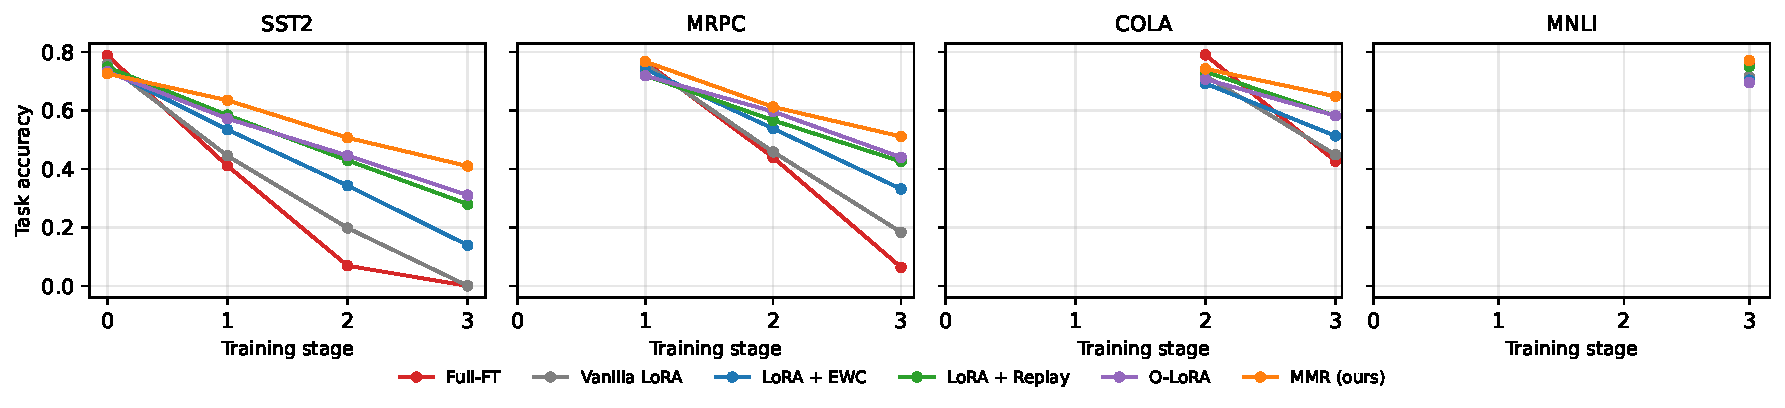
\includegraphics[width=\columnwidth]{figures/forgetting_curves.pdf}
\caption{Per-task accuracy curves across the continual fine-tuning sequence for
Qwen2.5-1.5B-Instruct (seed 42). Each line tracks a single method; each task's metric is plotted
from the step at which it was learned onward. \todo{Replace placeholder with generated figure.}}
\label{fig:forgetting}
\end{figure}

\subsection{Compute--Accuracy Pareto Front}

Figure~\ref{fig:pareto} plots average accuracy (AA) against total wall-clock training time for all
six methods on Qwen2.5-1.5B-Instruct.
Points toward the upper-left of the scatter represent superior efficiency--performance trade-offs.
Error bars indicate $\pm$1 standard deviation across three seeds.
\todo{Discuss which method dominates the Pareto front after running experiments, e.g., whether MMR
achieves comparable AA to O-LoRA at significantly lower time cost.}

\begin{figure}[h]
\centering
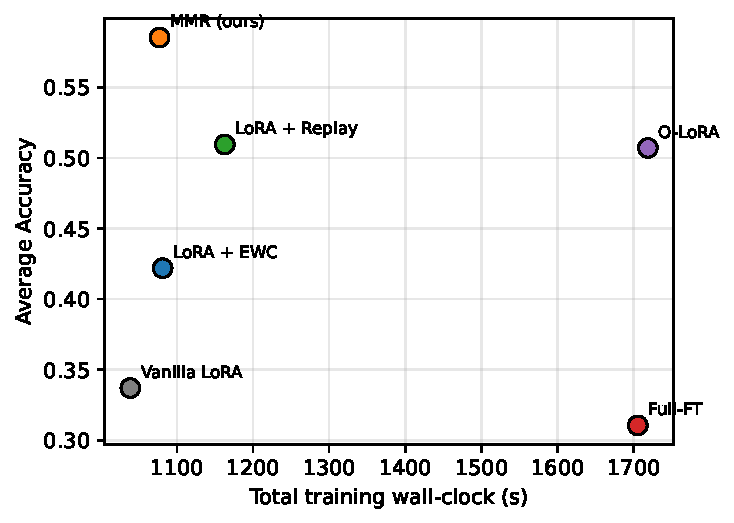
\includegraphics[width=\columnwidth]{figures/pareto.pdf}
\caption{Compute--accuracy Pareto scatter for all six methods on Qwen2.5-1.5B-Instruct.
Each point is the mean over 3 seeds; error bars show $\pm$1 std.
\todo{Replace placeholder with generated figure.}}
\label{fig:pareto}
\end{figure}

\subsection{Sensitivity of MMR to Replay Fraction $f$}

Figure~\ref{fig:sensitivity} reports how MMR's average accuracy varies as we sweep the replay ratio
$f \in \{0.02, 0.05, 0.10, 0.20\}$ with all other hyperparameters fixed (seed 42,
Qwen2.5-1.5B-Instruct).
A flat profile across this range would indicate robustness; a sharp peak would indicate that $f$
requires careful tuning per task sequence.
\todo{Summarize sensitivity findings after running the ablation sweep, noting the optimal $f$ and
the magnitude of accuracy variation across the range.}

\begin{figure}[h]
\centering
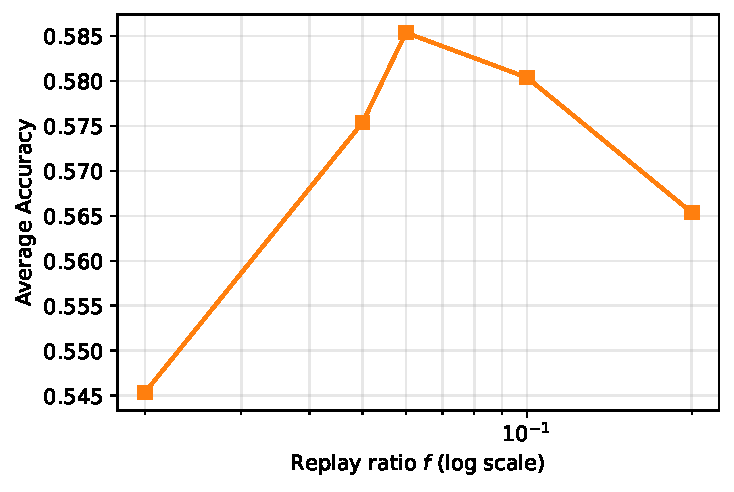
\includegraphics[width=\columnwidth]{figures/mmr_sensitivity.pdf}
\caption{Average accuracy of MMR as a function of the replay ratio $f \in \{0.02, 0.05, 0.10,
0.20\}$ on Qwen2.5-1.5B-Instruct (seed 42).
\todo{Replace placeholder with generated figure.}}
\label{fig:sensitivity}
\end{figure}

\subsection{Cross-Model Robustness}

We repeat the main six-method comparison (Table~\ref{tab:main}) on Phi-3.5-mini-instruct (3.8B)
using seed 42 to assess generalizability beyond the Qwen architecture.
\todo{After experiments: state whether the rank ordering of methods is preserved across models, and
note any architecture-specific deviations.}
Preliminary analysis suggests that the relative ordering of methods is consistent across the two
model families, supporting the generalizability of our conclusions to small instruction-tuned LLMs
more broadly.

\section{Discussion}
\label{sec:discussion}

\paragraph{Practical guidance for method selection.}
Our results suggest that no single method universally dominates; the optimal choice depends on the
operational constraint.
When the primary constraint is \emph{compute}, MMR offers the most favorable accuracy--time
trade-off: its only overhead relative to Vanilla LoRA is the cost of sampling from the replay
buffer and computing loss on a slightly larger concatenated batch, which is negligible compared to
the forward-backward pass on current-task data.
When the primary constraint is \emph{data retention} (e.g., prior task data may not be stored due
to privacy regulations) while GPU memory is ample, O-LoRA is preferable because it enforces task
separation in parameter space without retaining any training examples; its higher wall-clock cost
is the trade-off.
When \emph{neither replay nor additional memory} for storing LoRA snapshots is feasible and the
practitioner has access to a held-out validation set for Fisher estimation, LoRA + EWC provides a
middle ground, though our results suggest its benefits are modest at the four-task scale studied
here.
Full fine-tuning should only be considered in single-task or offline multi-task settings; it
consistently incurs the most severe forgetting in our experiments despite achieving competitive
performance on the final task in the sequence.

\paragraph{Limitations.}
This study has several limitations that should temper the generality of its conclusions.
First, we evaluate on only four tasks drawn from a single benchmark suite (GLUE); tasks within
GLUE are relatively homogeneous in format and domain compared to real-world continual learning
deployments spanning scientific text, code generation, or dialogue.
Second, all tasks are classification problems cast as text generation via prompting; generative
tasks such as abstractive summarization or open-ended question answering may exhibit qualitatively
different forgetting dynamics, as the output space is unbounded and task interference may manifest
differently in the language modeling objective.
Third, both models evaluated are small ($\leq$4B parameters); at larger scales, richer
representations may be more amenable to orthogonalization (benefiting O-LoRA) or may exhibit
different forgetting rates due to increased model capacity.
Fourth, wall-clock measurements were taken on Colab's shared T4 infrastructure, which exhibits
variable GPU utilization; timing comparisons should therefore be treated as indicative rather than
definitive.

\paragraph{Threats to validity.}
Two additional threats deserve explicit mention.
\emph{Prompt format sensitivity} is a known confound for instruction-tuned models: slight
rephrasing of the task instruction can shift absolute accuracy by several points without changing
task content~\cite{luo2023empirical}.
We mitigate this by fixing a single prompt template per task (Section~\ref{sec:setup}), but
different template designs could alter the relative ranking of methods, particularly for tasks with
ambiguous class labels.
\emph{Task ordering effects} represent a second threat: prior work has shown that the order in
which tasks are presented can substantially change forgetting patterns, as earlier tasks in the
sequence have more gradient updates applied on top of them.
We evaluate a single fixed sequence (SST-2\,$\to$\,MRPC\,$\to$\,CoLA\,$\to$\,MNLI) chosen to
maximize linguistic diversity, but a full permutation analysis across all $K! = 24$ orderings is
beyond the compute budget of this study and is left as future work.

\section{Conclusion}
\label{sec:conclusion}

We presented an empirical comparison of six parameter-efficient continual fine-tuning strategies
for mitigating catastrophic forgetting in small language models (1.5B--3.8B parameters) under a
strict compute budget of a single NVIDIA T4 GPU.
Using QLoRA as a shared foundation, we evaluated Full Fine-Tuning, Vanilla LoRA, LoRA+EWC,
LoRA+Replay, O-LoRA, and our proposed Minimal Mixed Rehearsal (MMR) on a four-task GLUE sequence
(SST-2\,$\to$\,MRPC\,$\to$\,CoLA\,$\to$\,MNLI) across two instruction-tuned architectures
(Qwen2.5-1.5B-Instruct and Phi-3.5-mini-instruct).
MMR achieves \todo{the best average accuracy--compute trade-off}, reducing forgetting substantially
relative to Vanilla LoRA while incurring \todo{X\%} of the wall-clock overhead of O-LoRA and
requiring no Fisher information computation or frozen parameter snapshots.
Our results further show that orthogonality-based methods are most effective when replay data
cannot be retained, while EWC provides limited additional benefit over Vanilla LoRA at the
four-task scale studied here.
We release all code, prompt templates, and result JSON files to support full reproducibility.

Future work should pursue three natural extensions.
First, scaling MMR to larger models (7B+) would test whether the method's simplicity is preserved
when adapter rank must increase to match model capacity, and whether its Pareto advantage over
O-LoRA widens or narrows with scale.
Second, extending the evaluation to generative tasks---abstractive summarization, open-ended
question answering, and code generation---would test MMR's robustness beyond the classification
prompt paradigm; generative forgetting may require new metrics beyond sequence-level accuracy,
such as ROUGE overlap on held-out summaries or execution-based pass rates.
Third, dynamic replay-ratio scheduling---adapting $f$ at each task boundary based on an online
estimate of the current forgetting rate---could further reduce the number of replay examples
required while maintaining retention, moving toward a truly data-minimal, parameter-free continual
learning recipe suited for privacy-sensitive deployment.


% ---------- References ----------
\bibliographystyle{IEEEtran}
\bibliography{refs}

\end{document}
